\chapter{Уравнения Максвелла, ковариантность и электромагнитные волны}

\lectureoverview{Электрическое и магнитное поля действуют на заряженное вещество через силу Лоренца, но вещество должно также создавать поля и изменять их конфигурацию. Мы сформулируем эту обратную половину электромагнетизма, покажем, что уравнения Максвелла лоренц-ковариантны, выведем их волновые решения, а затем вернём заряд и ток в форме, которая делает локальный закон сохранения явным. На протяжении всей лекции мы используем единицы, в которых \(c=1\).}

\section{Другая половина электромагнетизма}

Начнём с той части предмета, которая уже нам известна. Если частица с зарядом \(q\) движется со скоростью \(\mathbf v\) в электрическом и магнитном полях, то сила равна
\begin{equation}
\mathbf F=q\bigl(\mathbf E+\mathbf v\times\mathbf B\bigr).
\label{eq:lorentz-force-three}
\end{equation}
Множитель \(q\) принципиально необходим. Незаряженная частица не испытывает электромагнитной силы. Электрическое поле даёт вклад даже тогда, когда частица мгновенно покоится, тогда как магнитный вклад зависит от её движения.

Уравнение~\eqref{eq:lorentz-force-three} говорит нам, что делают с веществом заданные поля. Оно не говорит, чем определяются сами поля. Что создаёт электрическое поле вокруг одного объекта, магнитное поле вокруг другого или волну, движущуюся через пустое пространство? На эти вопросы отвечают уравнения Максвелла.

\begin{figure}[H]
\centering
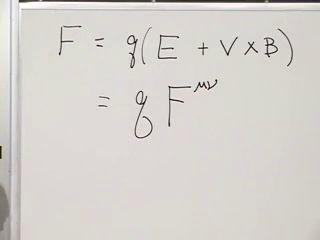
\includegraphics[width=0.62\textwidth]{lecture_58_figure_02.png}
\caption{Трёхвекторная сила Лоренца и начало её тензорной переформулировки.}
\lectureframe{00:05:49}
\end{figure}

Релятивистская форма закона силы предвосхищает обозначения, которые нам понадобятся:
\begin{equation}
f^\mu=qF^\mu{}_{\nu}u^\nu.
\label{eq:lorentz-force-four}
\end{equation}
Здесь \(u^\nu\) — это четырёхскорость, \(f^\mu\) — четырёхсила, а \(F^{\mu\nu}\) — антисимметричный тензор, составленный из \(\mathbf E\) и \(\mathbf B\). На доске сначала показано лишь схематическое начало этого выражения; свёртка с \(u^\nu\) даёт недостающий вектор, необходимый, чтобы остался один свободный индекс силы.

Есть физическая причина, по которой вещество должно воздействовать обратно на поле. Электромагнитная волна может налететь на заряд, ускорить его и передать ему энергию. Если бы поле могло воздействовать на заряд, а заряд никак не мог бы воздействовать на поле, не было бы места, откуда эта энергия была бы изъята. Принцип действия и противодействия — не весь аргумент, но закон сохранения энергии делает такую взаимную связь неизбежной.

\section{Изменяющийся источник порождает возмущение}

Точечный заряд создаёт электрическое поле, направленное наружу от его положения или внутрь к нему. Ток в проводе--поток заряженных частиц--создаёт магнитное поле, циркулирующее вокруг провода. Эти знакомые статические картины уже показывают две разные геометрические структуры: электрический поток исходит от заряда, тогда как линии магнитного поля обвивают ток.

Теперь резко переместим точечный заряд. Вблизи его нового положения электрическое поле должно начать перестраиваться, но далёкий наблюдатель не может узнать об этом движении мгновенно. Вдали старое поле сохраняется до тех пор, пока сигнал не успеет прийти. Между ближней и дальней областями находится движущийся фронт, на котором поле изменяется. Эта движущаяся перестройка и есть электромагнитное возмущение.

Если заряд заставить двигаться туда и обратно, последовательные перестройки будут следовать одна за другой и образуют электромагнитную волну. В этом и состоит элементарная функция антенны: колеблющийся электрический ток посылает наружу возмущение поля. Обращение тока в проводе даёт магнитный вариант того же рассуждения. Циркуляция \(\mathbf B\) должна обратиться, но это обращение распространяется, а не возникает сразу повсюду.

Эта причинная картина ставит перед уравнениями Максвелла две задачи. Они должны описывать, как заряд и ток служат источниками полей, и должны допускать распространение изменений в этих полях не быстрее света. Вторая задача одновременно является и проверкой теории относительности. Если уравнения Максвелла имеют один и тот же вид в каждой инерциальной системе отсчёта и влекут определённую скорость волны, то каждая инерциальная система должна выводить из них одну и ту же скорость.

\section{Повторение релятивистского волнового уравнения}

Прежде чем переходить к векторным полям, рассмотрим скалярное поле \(\phi(\mathbf x,t)\), одно число в каждой точке пространства-времени. Уравнение с первыми производными
\begin{equation}
\partial_\mu\phi=0
\end{equation}
означало бы, что все производные по координатам пространства-времени равны нулю. Поле было бы постоянным и потому не могло бы нести волну. Нетривиальное релятивистское волновое уравнение использует две производные:
\begin{equation}
\partial_\mu\partial^\mu\phi=0.
\end{equation}
При используемом здесь соглашении о знаках
\begin{equation}
\left(\partial_t^2-\partial_x^2-\partial_y^2-\partial_z^2\right)\phi=0,
\label{eq:scalar-wave-four}
\end{equation}
или, более компактно,
\begin{equation}
\left(\partial_t^2-\nabla^2\right)\phi=0.
\end{equation}
Выбор \(c=1\) делает единицы времени и расстояния согласованными. При восстановлении обычных единиц множитель \(1/c^2\) появился бы при второй производной по времени.

Для волны, распространяющейся вдоль оси \(z\), поле зависит от \(z\) и \(t\), а не от \(x\) или \(y\). Уравнение~\eqref{eq:scalar-wave-four} принимает вид
\begin{equation}
\left(\partial_t^2-\partial_z^2\right)\phi=0.
\label{eq:scalar-wave-one}
\end{equation}

\begin{figure}[H]
\centering
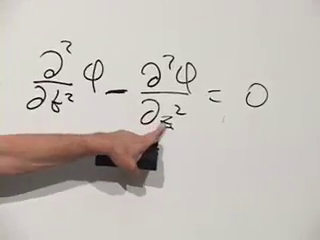
\includegraphics[width=0.56\textwidth]{lecture_58_figure_04.png}
\caption{Одномерное скалярное волновое уравнение, используемое в качестве модели для электромагнитных волн.}
\lectureframe{00:47:03}
\end{figure}

Его общий вид бегущей волны таков:
\begin{equation}
\phi(z,t)=f(z-t)+g(z+t).
\end{equation}
Профиль \(f(z-t)\) движется в сторону возрастания \(z\), поскольку точка фиксированной фазы удовлетворяет \(z-t=\text{constant}\). Профиль \(g(z+t)\) движется в противоположном направлении. Ничто не требует, чтобы какой-либо из этих профилей был синусоидальным; любая достаточно гладкая форма распространяется без изменения формы.

Синусоиды, однако, удобны:
\begin{equation}
\phi(z,t)=A\cos\!\bigl(k(z-t)\bigr).
\end{equation}
Волновое число \(k\) определяет длину волны,
\begin{equation}
\lambda=\frac{2\pi}{k}.
\end{equation}
Большое \(k\) даёт быстрые пространственные осцилляции и малую длину волны; малое \(k\) даёт большую длину волны. Эти же профили вскоре станут компонентами \(\mathbf E\) и \(\mathbf B\).

\section{Векторный анализ, необходимый для уравнений Максвелла}

Уравнения Максвелла записываются с помощью скалярных произведений, векторных произведений, дивергенции и ротора. Стоит один раз заново восстановить эти обозначения, потому что последующие покомпонентные вычисления используют именно такие структуры.

Для обычных трёхмерных векторов \(\mathbf a\) и \(\mathbf b\) скалярное произведение есть скаляр
\begin{equation}
\mathbf a\cdot\mathbf b
=a_xb_x+a_yb_y+a_zb_z.
\end{equation}
Векторное произведение — ещё один вектор,
\begin{align}
(\mathbf a\times\mathbf b)_x&=a_yb_z-a_zb_y,\\
(\mathbf a\times\mathbf b)_y&=a_zb_x-a_xb_z,\\
(\mathbf a\times\mathbf b)_z&=a_xb_y-a_yb_x.
\end{align}
Остальные компоненты следуют из циклического порядка \(x\to y\to z\to x\).

Введём дифференциальный оператор
\begin{equation}
\boldsymbol\nabla=
\left(\partial_x,\partial_y,\partial_z\right).
\end{equation}
Его компоненты являются операторами, а не обычными числами, но схемы скалярного и векторного произведений всё равно можно использовать. Для векторного поля \(\mathbf A\)
\begin{equation}
\boldsymbol\nabla\cdot\mathbf A
=\partial_xA_x+\partial_yA_y+\partial_zA_z
\label{eq:divergence}
\end{equation}
есть дивергенция, тогда как
\begin{align}
(\boldsymbol\nabla\times\mathbf A)_x
 &=\partial_yA_z-\partial_zA_y,\\
(\boldsymbol\nabla\times\mathbf A)_y
 &=\partial_zA_x-\partial_xA_z,\\
(\boldsymbol\nabla\times\mathbf A)_z
 &=\partial_xA_y-\partial_yA_x
\label{eq:curl}
\end{align}
есть компоненты ротора.

Геометрия не менее важна, чем формулы. Векторное поле имеет положительную дивергенцию там, где кажется, что оно растекается наружу от источника. Оно имеет ротор там, где циркулирует. Радиальное электрическое поле точечного заряда иллюстрирует дивергенцию; магнитное поле, обвивающее провод с током, иллюстрирует ротор. Пространственно постоянное векторное поле не имеет ни того, ни другого.

\section{Уравнения Максвелла в вакууме}

В отсутствие заряда и тока уравнения Максвелла имеют вид
\begin{align}
\boldsymbol\nabla\times\mathbf E&=-\partial_t\mathbf B,
\label{eq:faraday-vac}\\
\boldsymbol\nabla\cdot\mathbf B&=0,
\label{eq:gauss-b-vac}\\
\boldsymbol\nabla\times\mathbf B&=\partial_t\mathbf E,
\label{eq:ampere-vac}\\
\boldsymbol\nabla\cdot\mathbf E&=0.
\label{eq:gauss-e-vac}
\end{align}
Два уравнения на ротор почти переходят друг в друга при замене \(\mathbf E\) на \(\mathbf B\), но их различает существенный знак минус. Два уравнения на дивергенцию говорят, что ни одно из полей не имеет источника в рассматриваемой области вакуума. Магнитная дивергенция остаётся нулевой даже после того, как электрические источники будут возвращены; обычный электромагнетизм не содержит магнитного заряда.

\begin{figure}[H]
\centering
\includegraphics[width=0.76\textwidth]{lecture_58_figure_06.png}
\caption{Четыре вакуумных уравнения Максвелла, записанные так, чтобы показать почти симметрию между электрическим и магнитным полями.}
\lectureframe{00:27:30}
\end{figure}

Плотность заряда \(\rho\) впоследствии заменит нуль в правой части уравнения~\eqref{eq:gauss-e-vac}, а плотность тока \(\mathbf J\) войдёт в уравнение~\eqref{eq:ampere-vac}. Пока временно отложим эти члены. Уравнения без источников выявляют структуру преобразований и волновой механизм при минимуме лишних членов.

Они также делают ещё острее эйнштейновскую проблему. Наблюдатель, следующий за волной в галилеевой кинематике, ожидал бы вычесть скорости и измерить меньшую скорость волны. Однако если одни и те же уравнения Максвелла выполняются в каждой инерциальной системе отсчёта, то каждый наблюдатель выводит из них одну и ту же единичную скорость волны. Выход состоит не в том, чтобы изменять волновое уравнение от системы к системе. Он состоит в том, чтобы использовать преобразование Лоренца и выразить уравнения Максвелла через объекты, законы преобразования которых уже известны.

\section{Электрическое и магнитное поля как единый тензор}

Электрическое и магнитное поля объединяются в антисимметричный тензор поля
\begin{equation}
F^{\mu\nu}=
\begin{pmatrix}
0   & -E_x & -E_y & -E_z\\
E_x & 0    & -B_z & B_y\\
E_y & B_z  & 0    & -B_x\\
E_z & -B_y & B_x  & 0
\end{pmatrix},
\label{eq:l0203-field-tensor}
\end{equation}
где порядок строк и столбцов таков: \(t,x,y,z\). Антисимметрия,
\begin{equation}
F^{\mu\nu}=-F^{\nu\mu},
\end{equation}
заставляет диагональные элементы обращаться в нуль и определяет нижнюю половину матрицы по верхней. Временнó-пространственные элементы содержат \(\mathbf E\); чисто пространственные элементы содержат \(\mathbf B\).

\begin{figure}[H]
\centering
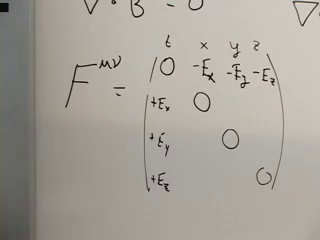
\includegraphics[width=0.58\textwidth]{lecture_58_figure_03.png}
\caption{Полный тензор электромагнитного поля, включая его электрические и магнитные компоненты.}
\lectureframe{00:32:05}
\end{figure}

Важность \(F^{\mu\nu}\) состоит не только в том, что шесть компонент поля помещаются в одну матрицу. При преобразовании Лоренца он преобразуется как тензор второго ранга. Поэтому электрические и магнитные поля, измеряемые разными наблюдателями, смешиваются ровно так, как требуется, чтобы весь объект преобразовывался согласованно.

Существует второй антисимметричный тензор — дуальный тензор поля \(\widetilde F^{\mu\nu}\). При принятой здесь конвенции он получается из уравнения~\eqref{eq:l0203-field-tensor} заменой
\begin{equation}
\mathbf E\longmapsto-\mathbf B,
\qquad
\mathbf B\longmapsto\mathbf E.
\label{eq:dual-replacement}
\end{equation}
Отсюда
\begin{equation}
\widetilde F^{\mu\nu}=
\begin{pmatrix}
0    & B_x  & B_y  & B_z\\
-B_x & 0    & -E_z & E_y\\
-B_y & E_z  & 0    & -E_x\\
-B_z & -E_y & E_x  & 0
\end{pmatrix}.
\label{eq:dual-tensor}
\end{equation}
Знак в уравнении~\eqref{eq:dual-replacement} существен. В лекции сначала пытаются выполнить эту перестановку на словах, замечают несоответствие знака и исправляют его, прежде чем завершить матрицу.

\begin{figure}[H]
\centering
\includegraphics[width=0.58\textwidth]{lecture_58_figure_07.png}
\caption{Дуальный тензор строится перестановкой электрических и магнитных компонент с требуемым знаком.}
\lectureframe{00:35:45}
\end{figure}

\section{Ковариантные уравнения в вакууме}

Каждое уравнение Максвелла содержит одну производную. Если начать с тензора ранга два и свернуть по одному индексу производной, останется один свободный индекс, поэтому естественными ковариантными кандидатами являются
\begin{align}
\partial_\mu F^{\mu\nu}&=0,
\label{eq:maxwell-covariant-vac}\\
\partial_\mu\widetilde F^{\mu\nu}&=0.
\label{eq:maxwell-dual-vac}
\end{align}
Для каждого фиксированного значения \(\nu\) уравнение~\eqref{eq:maxwell-covariant-vac} представляет собой одно уравнение. Поскольку \(\nu\) может принимать значения \(t,x,y,z\), оно объединяет четыре скалярных уравнения. Уравнение~\eqref{eq:maxwell-dual-vac} объединяет ещё четыре. Это соответствует двум векторным уравнениям на ротор и двум скалярным уравнениям на дивергенцию в исходном списке.

Компактная запись полезна лишь тогда, когда она воспроизводит знакомые уравнения. Возьмём \(\nu=z\):
\begin{align}
\partial_\mu F^{\mu z}
&=\partial_tF^{tz}
  +\partial_xF^{xz}
  +\partial_yF^{yz}
  +\partial_zF^{zz}\\
&=-\partial_tE_z+\partial_xB_y-\partial_yB_x\\
&=-\partial_tE_z+
  \bigl(\boldsymbol\nabla\times\mathbf B\bigr)_z.
\end{align}
Член \(F^{zz}\) обращается в нуль по антисимметрии. Приравнивание результата к нулю даёт \(z\)-компоненту
\begin{equation}
\boldsymbol\nabla\times\mathbf B=\partial_t\mathbf E.
\end{equation}
\(x\)- и \(y\)-компоненты получаются циклической перестановкой индексов.

\begin{figure}[H]
\centering
\includegraphics[width=0.76\textwidth]{lecture_58_figure_08.png}
\caption{Покомпонентное разложение ковариантного уравнения поля; диагональный элемент тензора обращается в нуль, а остальные члены восстанавливают уравнения Максвелла.}
\lectureframe{00:43:30}
\end{figure}

Теперь возьмём временную компоненту:
\begin{align}
\partial_\mu F^{\mu t}
&=\partial_tF^{tt}
  +\partial_xF^{xt}
  +\partial_yF^{yt}
  +\partial_zF^{zt}\\
&=\partial_xE_x+\partial_yE_y+\partial_zE_z\\
&=\boldsymbol\nabla\cdot\mathbf E.
\end{align}
Следовательно, это даёт уравнение~\eqref{eq:gauss-e-vac}. Те же проверки для дуального тензора дают
\(\boldsymbol\nabla\cdot\mathbf B=0\) и
\(\boldsymbol\nabla\times\mathbf E=-\partial_t\mathbf B\).

Компактные уравнения теперь установлены, а не просто угаданы. Их структура со свободным индексом делает их четырёхвекторными уравнениями, поэтому преобразование Лоренца меняет их компоненты, но не их форму. Именно в этом точном смысле вакуумные уравнения Максвелла одинаковы во всех инерциальных системах отсчёта.

\section{От уравнений первого порядка к волне}

Уравнения Максвелла содержат только первые производные, тогда как волновое уравнение содержит вторые производные. Кажущееся несоответствие устраняется тем, что теория Максвелла связывает два поля. Пару уравнений первого порядка для \(\mathbf E\) и \(\mathbf B\) можно объединить в уравнение второго порядка для любого из этих полей по отдельности.

Продифференцируем уравнение~\eqref{eq:ampere-vac} по времени:
\begin{equation}
\partial_t^2\mathbf E
=\boldsymbol\nabla\times\partial_t\mathbf B.
\end{equation}
Закон Фарадея даёт временную производную \(\mathbf B\),
\begin{equation}
\partial_t\mathbf B=-\boldsymbol\nabla\times\mathbf E,
\end{equation}
и потому
\begin{equation}
\partial_t^2\mathbf E
=-\boldsymbol\nabla\times
  \bigl(\boldsymbol\nabla\times\mathbf E\bigr).
\label{eq:double-curl}
\end{equation}

На доске подробно разбирается одна компонента, а не используется заученное тождество. Для \(x\)-компоненты
\begin{align}
\bigl[\boldsymbol\nabla\times
(\boldsymbol\nabla\times\mathbf E)\bigr]_x
&=\partial_y(\boldsymbol\nabla\times\mathbf E)_z
 -\partial_z(\boldsymbol\nabla\times\mathbf E)_y\\
&=\partial_y(\partial_xE_y-\partial_yE_x)\\
&\quad-\partial_z(\partial_zE_x-\partial_xE_z)\\
&=\partial_x(\partial_yE_y+\partial_zE_z)
 -\partial_y^2E_x\\
&\quad-\partial_z^2E_x.
\end{align}
Прибавим и вычтем \(\partial_x^2E_x\), чтобы выделить дивергенцию:
\begin{align}
\bigl[\boldsymbol\nabla\times
(\boldsymbol\nabla\times\mathbf E)\bigr]_x
&=\partial_x(\boldsymbol\nabla\cdot\mathbf E)
 -\nabla^2E_x.
\label{eq:double-curl-x}
\end{align}
В вакууме \(\boldsymbol\nabla\cdot\mathbf E=0\). Объединяя
уравнения~\eqref{eq:double-curl} и \eqref{eq:double-curl-x}, получаем
\begin{equation}
\left(\partial_t^2-\nabla^2\right)E_x=0.
\label{eq:ex-wave}
\end{equation}

\begin{figure}[H]
\centering
\includegraphics[width=0.72\textwidth]{lecture_58_figure_09.png}
\caption{Покомпонентный расчёт приводит к волновому уравнению для \(E_x\).}
\lectureframe{00:57:10}
\end{figure}

Тот же расчёт применим к \(E_y\) и \(E_z\), а аналогичное исключение даёт
\begin{equation}
\left(\partial_t^2-\nabla^2\right)\mathbf B=0.
\end{equation}
Следовательно, электрическое и магнитное поля могут распространяться в пустом пространстве в виде волн. В используемых здесь единицах их скорость равна единице, а после восстановления обычных единиц она равна \(c\).

\section{Плоская волна и её поляризация}

Построим простую волну, распространяющуюся в положительном направлении \(z\):
\begin{equation}
\mathbf E(z,t)
=\widehat{\mathbf x}\,E_0
  \cos\!\bigl(k(z-t)\bigr).
\label{eq:plane-e}
\end{equation}
Её профиль сдвигается вдоль \(z\), не меняя формы. Поскольку электрическое поле направлено вдоль оси \(x\), волна линейно поляризована в направлении \(x\). Мы выбрали \(E_y=0\) только для простоты примера; можно было бы включить и вторую поперечную поляризацию.

Продольная компонента не является столь же произвольной. Поскольку волна зависит только от \(z\) и \(t\),
\begin{equation}
\boldsymbol\nabla\cdot\mathbf E
=\partial_zE_z=0.
\end{equation}
Следовательно, \(E_z\) может быть постоянной, но не может содержать меняющийся волновой профиль. Однородное фоновое поле можно независимо наложить или убрать; оно не является частью распространяющегося излучения. Сама волна поперечна:
\begin{equation}
\mathbf E_{\mathrm{wave}}\cdot\widehat{\mathbf z}=0.
\end{equation}

Магнитное поле определяется законом Фарадея. Для уравнения~\eqref{eq:plane-e} единственная ненулевая компонента \(\boldsymbol\nabla\times\mathbf E\) — это \(y\)-компонента,
\begin{equation}
(\boldsymbol\nabla\times\mathbf E)_y=\partial_zE_x.
\end{equation}
Следовательно, \(\partial_t\mathbf B\) направлена вдоль \(y\), и совместимым выбором будет
\begin{equation}
\mathbf B(z,t)
=\widehat{\mathbf y}\,E_0
  \cos\!\bigl(k(z-t)\bigr).
\label{eq:plane-b}
\end{equation}
В этих единицах амплитуды электрического и магнитного полей равны. Их ориентация подчиняется соотношению
\begin{equation}
\mathbf E\perp\mathbf B,
\qquad
\mathbf E\perp\widehat{\mathbf z},
\qquad
\mathbf B\perp\widehat{\mathbf z},
\qquad
\mathbf E\times\mathbf B\parallel\widehat{\mathbf z}.
\end{equation}

\begin{figure}[H]
\centering
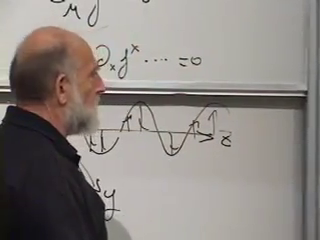
\includegraphics[width=0.70\textwidth]{lecture_58_figure_05.png}
\caption{Завершённый рисунок на доске поперечной электромагнитной волны: электрические и магнитные колебания перпендикулярны друг другу и направлению распространения.}
\lectureframe{01:05:25}
\end{figure}

\begin{figure}[H]
\centering
\scalebox{0.90}{%
\begin{tikzpicture}[x=1cm,y=1cm,>=Latex]
  \draw[->,thick] (0,0) -- (8.2,0) node[right] {$z$};
  \draw[->,thick] (0,-1.6) -- (0,1.7) node[above] {$x$};
  \draw[->,thick] (0,0) -- (-1.15,-0.8) node[below left] {$y$};
  \draw[blue!70!black,thick,domain=0:7.5,samples=120]
    plot (\x,{0.95*sin(90*\x)});
  \foreach \z/\s in {0.8/1,2.8/-1,4.8/1,6.8/-1}{
    \draw[->,green!45!black,thick]
      (\z,0) -- ++({-0.55*\s},{-0.38*\s});
  }
  \node[blue!70!black] at (6.9,1.25) {$\mathbf E$};
  \node[green!45!black] at (5.2,-1.05) {$\mathbf B$};
  \draw[->,very thick] (6.2,1.55) -- (7.7,1.55)
    node[midway,above] {propagation};
\end{tikzpicture}
}
\caption{Поля \(\mathbf E\) и \(\mathbf B\) перпендикулярны друг другу и направлению распространения.}
\end{figure}

Таков характер света и всего электромагнитного излучения в вакууме. Поскольку уравнения, из которых получена эта волна, лоренц-ковариантны, другой инерциальный наблюдатель тоже описывает электромагнитную волну, движущуюся со скоростью \(c\), с поперечными электрическим и магнитным полями.

\section{Плотность заряда и плотность тока}

Теперь мы возвращаем источники, которые были временно оставлены в стороне. Когда в некоторой области находится много заряженных частиц, полезно перейти к их грубозернистому описанию в виде непрерывной плотности заряда
\begin{equation}
\rho(\mathbf x,t)=\frac{dQ}{dV}.
\end{equation}
Это приближение похоже на рассмотрение воды как сплошной жидкости, хотя она состоит из молекул. Положительные и отрицательные заряды вносят вклады с противоположными знаками, так что \(\rho\) — это суммарный заряд на единицу объёма.

Заряд в выбранной области \(V\) равен
\begin{equation}
Q_V(t)=\int_V\rho(\mathbf x,t)\,dV.
\label{eq:charge-volume}
\end{equation}
Плотность может зависеть от положения и времени. Скопление заряда может уйти от точки, изменив там локальную плотность. Однако она не может изменяться произвольным образом. В природе электрический заряд сохраняется.

Одного лишь глобального закона сохранения было бы недостаточно. Он допускал бы, что заряд исчезает с Земли и в то же мгновение появляется на Марсе, тогда как полный заряд остаётся неизменным. Более сильное утверждение является локальным: заряд может покинуть одно место и попасть в другое только посредством потока через промежуточное пространство.

Чтобы описать этот поток, рассмотрим бесконечно малый ориентированный элемент поверхности
\begin{equation}
d\boldsymbol\sigma=\widehat{\mathbf n}\,d\sigma.
\end{equation}
Его модуль равен площади, а его направление перпендикулярно поверхности. Плотность тока \(\mathbf J\) определяется так, что заряд, пересекающий этот элемент в единицу времени, равен
\begin{equation}
\frac{dQ}{dt}=\mathbf J\cdot d\boldsymbol\sigma.
\label{eq:current-flux-element}
\end{equation}
Модуль \(\mathbf J\) имеет размерность заряда на единицу площади в единицу времени, а его направление совпадает с направлением потока положительного заряда.

\begin{figure}[H]
\centering
\includegraphics[width=0.64\textwidth]{lecture_58_figure_10.png}
\caption{Ориентированный элемент площади и множитель потока \(d\boldsymbol\sigma\cdot\mathbf J\).}
\lectureframe{01:18:15}
\end{figure}

Скалярное произведение выделяет компоненту, нормальную к поверхности. Ток, касательный к поверхности, не пересекает её и даёт нулевой вклад. Ток, параллельный нормали, даёт максимальный поток при фиксированном модуле. Ток в проводе — один частный случай, но \(\mathbf J\) может также описывать заряд, текущий через лист или через всё трёхмерное пространство.

\section{Локальное сохранение и уравнение непрерывности}

Зафиксируем область \(V\) в пространстве и направим наружу каждый элемент её замкнутой границы \(\partial V\). Если имеется суммарный направленный наружу ток, заряд внутри уменьшается:
\begin{equation}
\frac{dQ_V}{dt}
=-\oint_{\partial V}\mathbf J\cdot d\boldsymbol\sigma.
\label{eq:integral-conservation}
\end{equation}
Знак минус имеет физическую, а не условную природу: положительный поток наружу уносит положительный заряд из области. Используя уравнение~\eqref{eq:charge-volume},
\begin{equation}
\int_V\partial_t\rho\,dV
=-\oint_{\partial V}\mathbf J\cdot d\boldsymbol\sigma.
\label{eq:integral-continuity-one}
\end{equation}

\begin{figure}[H]
\centering
\includegraphics[width=0.72\textwidth]{lecture_58_figure_11.png}
\caption{Закон сохранения для фиксированной области после преобразования поверхностного потока в объёмное соотношение.}
\lectureframe{01:29:00}
\end{figure}

Теорема Гаусса, также называемая теоремой о дивергенции, связывает поток через замкнутую поверхность с дивергенцией внутри неё:
\begin{equation}
\oint_{\partial V}\mathbf A\cdot d\boldsymbol\sigma
=\int_V\boldsymbol\nabla\cdot\mathbf A\,dV.
\label{eq:divergence-theorem}
\end{equation}
Можно представить себе скрытые трубы, подающие воду в точки внутри сосуда. Дивергенция измеряет локальную скорость, с которой вода выходит из концов труб; поверхностный интеграл измеряет полное количество воды, покидающей сосуд. Всё, что создаётся внутри как направленный наружу поток, в конце концов должно пересечь границу.

Применяя уравнение~\eqref{eq:divergence-theorem} к \(\mathbf J\), получаем
\begin{equation}
\int_V
\left(\partial_t\rho+\boldsymbol\nabla\cdot\mathbf J\right)dV=0.
\end{equation}
Это соотношение верно для любой области \(V\). Следовательно, подынтегральное выражение должно обращаться в нуль в каждой точке:
\begin{equation}
\boxed{\partial_t\rho+\boldsymbol\nabla\cdot\mathbf J=0.}
\label{eq:continuity-three}
\end{equation}

\begin{figure}[H]
\centering
\includegraphics[width=0.72\textwidth]{lecture_58_figure_12.png}
\caption{Локальное уравнение непрерывности, записанное покомпонентно.}
\lectureframe{01:29:50}
\end{figure}

Уравнение~\eqref{eq:continuity-three} выражает в точности то, чего требует локальное сохранение. Если плотность заряда уменьшается в точке или внутри малой области, ток должен расходиться наружу из неё. Если ток сходится внутрь, плотность заряда увеличивается.

Плотность заряда и плотность тока естественно образуют четырёхток
\begin{equation}
J^\mu=(\rho,J_x,J_y,J_z)
\label{eq:four-current}
\end{equation}
в единицах \(c=1\). Уравнение непрерывности принимает вид лоренц-скалярного уравнения
\begin{equation}
\partial_\mu J^\mu=0.
\label{eq:continuity-four}
\end{equation}
Поток релятивистского распределения должен преобразовываться как четырёхвектор, так же как четырёхскорость отдельной частицы. Уравнение~\eqref{eq:continuity-four} делает локальное сохранение заряда справедливым во всех инерциальных системах отсчёта.

\section{Уравнения Максвелла с источниками}

При восстановлении заряда и тока получаем
\begin{align}
\boldsymbol\nabla\cdot\mathbf E&=\rho,
\label{eq:gauss-e-source}\\
\boldsymbol\nabla\cdot\mathbf B&=0,\\
\boldsymbol\nabla\times\mathbf E&=-\partial_t\mathbf B,\\
\boldsymbol\nabla\times\mathbf B&=\partial_t\mathbf E+\mathbf J.
\label{eq:ampere-source}
\end{align}
Уравнения с электрическими источниками сводятся к
\begin{equation}
\boxed{\partial_\mu F^{\mu\nu}=J^\nu,}
\label{eq:maxwell-source-covariant}
\end{equation}
тогда как магнитная пара без источников сохраняет вид
\begin{equation}
\boxed{\partial_\mu\widetilde F^{\mu\nu}=0.}
\label{eq:maxwell-dual-source}
\end{equation}

\begin{figure}[H]
\centering
\includegraphics[width=0.78\textwidth]{lecture_58_figure_13.png}
\caption{Уравнения Максвелла с источниками рядом с их ковариантной формой \(\partial_\mu F^{\mu\nu}=J^\nu\).}
\lectureframe{01:34:00}
\end{figure}

Временная компонента уравнения~\eqref{eq:maxwell-source-covariant} имеет вид
\begin{equation}
\partial_\mu F^{\mu t}=J^t=\rho,
\end{equation}
а уже выполненное покомпонентное вычисление превращает его левую часть в
\(\boldsymbol\nabla\cdot\mathbf E\). Три пространственные компоненты воспроизводят
\(\boldsymbol\nabla\times\mathbf B=\partial_t\mathbf E+\mathbf J\).

Есть и полезная проверка на согласованность. Применяя \(\partial_\nu\) к
уравнению~\eqref{eq:maxwell-source-covariant}, получаем
\begin{equation}
\partial_\nu J^\nu
=\partial_\nu\partial_\mu F^{\mu\nu}=0,
\end{equation}
поскольку две производные симметричны при \(\mu\leftrightarrow\nu\), тогда как \(F^{\mu\nu}\) антисимметричен.\editorialnote{Эта краткая проверка на согласованность следует из ковариантного уравнения и явно показывает, почему уравнения Максвелла с источниками автоматически удовлетворяют уравнению непрерывности.}

Теперь взаимная структура завершена. Тензорный закон силы
\(f^\mu=qF^\mu{}_\nu u^\nu\) описывает, как поля действуют на заряд, а
уравнение~\eqref{eq:maxwell-source-covariant} описывает, как заряд и ток порождают поля. Оба являются тензорными уравнениями. В вакууме те же уравнения поля дают поперечные волны, распространяющиеся со скоростью \(c\). Поэтому ковариантность Лоренца и уравнение электромагнитной волны сходятся в той точке, которая и мотивировала это построение: каждый инерциальный наблюдатель получает одни и те же законы электромагнетизма и одну и ту же скорость света.
